% Options for packages loaded elsewhere
\PassOptionsToPackage{unicode}{hyperref}
\PassOptionsToPackage{hyphens}{url}
%
\documentclass[
]{book}
\usepackage{amsmath,amssymb}
\usepackage{lmodern}
\usepackage{iftex}
\ifPDFTeX
  \usepackage[T1]{fontenc}
  \usepackage[utf8]{inputenc}
  \usepackage{textcomp} % provide euro and other symbols
\else % if luatex or xetex
  \usepackage{unicode-math}
  \defaultfontfeatures{Scale=MatchLowercase}
  \defaultfontfeatures[\rmfamily]{Ligatures=TeX,Scale=1}
\fi
% Use upquote if available, for straight quotes in verbatim environments
\IfFileExists{upquote.sty}{\usepackage{upquote}}{}
\IfFileExists{microtype.sty}{% use microtype if available
  \usepackage[]{microtype}
  \UseMicrotypeSet[protrusion]{basicmath} % disable protrusion for tt fonts
}{}
\makeatletter
\@ifundefined{KOMAClassName}{% if non-KOMA class
  \IfFileExists{parskip.sty}{%
    \usepackage{parskip}
  }{% else
    \setlength{\parindent}{0pt}
    \setlength{\parskip}{6pt plus 2pt minus 1pt}}
}{% if KOMA class
  \KOMAoptions{parskip=half}}
\makeatother
\usepackage{xcolor}
\usepackage{color}
\usepackage{fancyvrb}
\newcommand{\VerbBar}{|}
\newcommand{\VERB}{\Verb[commandchars=\\\{\}]}
\DefineVerbatimEnvironment{Highlighting}{Verbatim}{commandchars=\\\{\}}
% Add ',fontsize=\small' for more characters per line
\usepackage{framed}
\definecolor{shadecolor}{RGB}{248,248,248}
\newenvironment{Shaded}{\begin{snugshade}}{\end{snugshade}}
\newcommand{\AlertTok}[1]{\textcolor[rgb]{0.94,0.16,0.16}{#1}}
\newcommand{\AnnotationTok}[1]{\textcolor[rgb]{0.56,0.35,0.01}{\textbf{\textit{#1}}}}
\newcommand{\AttributeTok}[1]{\textcolor[rgb]{0.77,0.63,0.00}{#1}}
\newcommand{\BaseNTok}[1]{\textcolor[rgb]{0.00,0.00,0.81}{#1}}
\newcommand{\BuiltInTok}[1]{#1}
\newcommand{\CharTok}[1]{\textcolor[rgb]{0.31,0.60,0.02}{#1}}
\newcommand{\CommentTok}[1]{\textcolor[rgb]{0.56,0.35,0.01}{\textit{#1}}}
\newcommand{\CommentVarTok}[1]{\textcolor[rgb]{0.56,0.35,0.01}{\textbf{\textit{#1}}}}
\newcommand{\ConstantTok}[1]{\textcolor[rgb]{0.00,0.00,0.00}{#1}}
\newcommand{\ControlFlowTok}[1]{\textcolor[rgb]{0.13,0.29,0.53}{\textbf{#1}}}
\newcommand{\DataTypeTok}[1]{\textcolor[rgb]{0.13,0.29,0.53}{#1}}
\newcommand{\DecValTok}[1]{\textcolor[rgb]{0.00,0.00,0.81}{#1}}
\newcommand{\DocumentationTok}[1]{\textcolor[rgb]{0.56,0.35,0.01}{\textbf{\textit{#1}}}}
\newcommand{\ErrorTok}[1]{\textcolor[rgb]{0.64,0.00,0.00}{\textbf{#1}}}
\newcommand{\ExtensionTok}[1]{#1}
\newcommand{\FloatTok}[1]{\textcolor[rgb]{0.00,0.00,0.81}{#1}}
\newcommand{\FunctionTok}[1]{\textcolor[rgb]{0.00,0.00,0.00}{#1}}
\newcommand{\ImportTok}[1]{#1}
\newcommand{\InformationTok}[1]{\textcolor[rgb]{0.56,0.35,0.01}{\textbf{\textit{#1}}}}
\newcommand{\KeywordTok}[1]{\textcolor[rgb]{0.13,0.29,0.53}{\textbf{#1}}}
\newcommand{\NormalTok}[1]{#1}
\newcommand{\OperatorTok}[1]{\textcolor[rgb]{0.81,0.36,0.00}{\textbf{#1}}}
\newcommand{\OtherTok}[1]{\textcolor[rgb]{0.56,0.35,0.01}{#1}}
\newcommand{\PreprocessorTok}[1]{\textcolor[rgb]{0.56,0.35,0.01}{\textit{#1}}}
\newcommand{\RegionMarkerTok}[1]{#1}
\newcommand{\SpecialCharTok}[1]{\textcolor[rgb]{0.00,0.00,0.00}{#1}}
\newcommand{\SpecialStringTok}[1]{\textcolor[rgb]{0.31,0.60,0.02}{#1}}
\newcommand{\StringTok}[1]{\textcolor[rgb]{0.31,0.60,0.02}{#1}}
\newcommand{\VariableTok}[1]{\textcolor[rgb]{0.00,0.00,0.00}{#1}}
\newcommand{\VerbatimStringTok}[1]{\textcolor[rgb]{0.31,0.60,0.02}{#1}}
\newcommand{\WarningTok}[1]{\textcolor[rgb]{0.56,0.35,0.01}{\textbf{\textit{#1}}}}
\usepackage{longtable,booktabs,array}
\usepackage{calc} % for calculating minipage widths
% Correct order of tables after \paragraph or \subparagraph
\usepackage{etoolbox}
\makeatletter
\patchcmd\longtable{\par}{\if@noskipsec\mbox{}\fi\par}{}{}
\makeatother
% Allow footnotes in longtable head/foot
\IfFileExists{footnotehyper.sty}{\usepackage{footnotehyper}}{\usepackage{footnote}}
\makesavenoteenv{longtable}
\usepackage{graphicx}
\makeatletter
\def\maxwidth{\ifdim\Gin@nat@width>\linewidth\linewidth\else\Gin@nat@width\fi}
\def\maxheight{\ifdim\Gin@nat@height>\textheight\textheight\else\Gin@nat@height\fi}
\makeatother
% Scale images if necessary, so that they will not overflow the page
% margins by default, and it is still possible to overwrite the defaults
% using explicit options in \includegraphics[width, height, ...]{}
\setkeys{Gin}{width=\maxwidth,height=\maxheight,keepaspectratio}
% Set default figure placement to htbp
\makeatletter
\def\fps@figure{htbp}
\makeatother
\setlength{\emergencystretch}{3em} % prevent overfull lines
\providecommand{\tightlist}{%
  \setlength{\itemsep}{0pt}\setlength{\parskip}{0pt}}
\setcounter{secnumdepth}{5}
\usepackage{booktabs}
\ifLuaTeX
  \usepackage{selnolig}  % disable illegal ligatures
\fi
\usepackage[]{natbib}
\bibliographystyle{plainnat}
\IfFileExists{bookmark.sty}{\usepackage{bookmark}}{\usepackage{hyperref}}
\IfFileExists{xurl.sty}{\usepackage{xurl}}{} % add URL line breaks if available
\urlstyle{same} % disable monospaced font for URLs
\hypersetup{
  pdftitle={CIÊNCIA DE DADOS COM LINGUAGEM R},
  pdfauthor={Richard Guilherme dos Santos},
  hidelinks,
  pdfcreator={LaTeX via pandoc}}

\title{CIÊNCIA DE DADOS COM LINGUAGEM R}
\author{Richard Guilherme dos Santos}
\date{}

\begin{document}
\maketitle

{
\setcounter{tocdepth}{1}
\tableofcontents
}
Bem vindos ao meu livro!

\hypertarget{introduuxe7uxe3o}{%
\chapter{Introdução}\label{introduuxe7uxe3o}}

Este livro tem como objetivo servir como guia para as aulas do curso Ciência de Dados com R. Nele apresentaremos os conceitos de:

\begin{enumerate}
\def\labelenumi{\arabic{enumi}.}
\tightlist
\item
  \textbf{Estatística Básica:} Nesta parte do curso abordaremos conceitos de estatística como variáveis, tipos de distribuições discretas e contínuas, medidas descritivas e distribuição normal.
\item
  \textbf{Manipulação de dados no R:} Neste tópico serão abordados as principais formas de manipulação de dados utilizando a linguagem R, com ênfase nas bibliotecas dplyr e tidyr. Além disso, abordaremos a criação de gráficos pelo pacote ggplot2.
\item
  \textbf{Modelos de Regressão Linear:} Parte final do curso, onde o aluno aprenderá sobre diagrama de dispersão, coeficiente de correlação linear, regressão linear simples, múltipla e regressão logística, ganhando a capacidade de começar a criar modelos utilizando a linguagem R.
\end{enumerate}

\hypertarget{introduuxe7uxe3o-a-probabilidade}{%
\chapter{Introdução a Probabilidade}\label{introduuxe7uxe3o-a-probabilidade}}

\hypertarget{introduuxe7uxe3o-ao-r}{%
\chapter{Introdução ao R}\label{introduuxe7uxe3o-ao-r}}

Aqui introduziremos alguns comandos da linguagem \texttt{R}, onde utilizamos funções para realizar operações que vão desde leitura e manipulação de dados a operações matemáticas.

Comecemos criando um vetor de números:

\begin{Shaded}
\begin{Highlighting}[]
\NormalTok{x }\OtherTok{\textless{}{-}} \FunctionTok{c}\NormalTok{(}\DecValTok{1}\NormalTok{,}\DecValTok{3}\NormalTok{,}\DecValTok{2}\NormalTok{,}\DecValTok{5}\NormalTok{)}
\CommentTok{\# x = c(1,3,2,5) \# Também podemos utilizar "=" para atribuir variáveis}
\NormalTok{x}
\end{Highlighting}
\end{Shaded}

\begin{verbatim}
## [1] 1 3 2 5
\end{verbatim}

O comando acima combina os números 1,3,2 e 5 em um vetor de números e os salva em um objeto denominado x. Escrevemos x para recebermos os atributos do vetor.

A partir disto podemos utilizar outras funções para calcularmos informações destes atributos, como o tamanho de um vetor:

\begin{Shaded}
\begin{Highlighting}[]
\FunctionTok{length}\NormalTok{(x)}
\end{Highlighting}
\end{Shaded}

\begin{verbatim}
## [1] 4
\end{verbatim}

ou sua média:

\begin{Shaded}
\begin{Highlighting}[]
\FunctionTok{mean}\NormalTok{(x)}
\end{Highlighting}
\end{Shaded}

\begin{verbatim}
## [1] 2.75
\end{verbatim}

Há outros tipos de objetos que podem ser criados quando trabalhamos com \texttt{R}. Os mais importantes para manipulação de dados são as matrizes:

\begin{Shaded}
\begin{Highlighting}[]
\NormalTok{mat }\OtherTok{=} \FunctionTok{matrix}\NormalTok{(}\AttributeTok{data =} \FunctionTok{c}\NormalTok{(}\DecValTok{1}\NormalTok{,}\DecValTok{2}\NormalTok{,}\DecValTok{3}\NormalTok{,}\DecValTok{4}\NormalTok{), }\AttributeTok{nrow =} \DecValTok{2}\NormalTok{, }\AttributeTok{ncol =} \DecValTok{2}\NormalTok{,}
           \AttributeTok{byrow =} \ConstantTok{TRUE}\NormalTok{)}
\NormalTok{mat}
\end{Highlighting}
\end{Shaded}

\begin{verbatim}
##      [,1] [,2]
## [1,]    1    2
## [2,]    3    4
\end{verbatim}

\begin{quote}
Funções aceitam os mais diversos tipos de argumentos. Para termos uma ideia de quais utilizarmos e seus respectivos atributos devemos fazer consultas em suas bibliotecas:

\begin{Shaded}
\begin{Highlighting}[]
\FunctionTok{help}\NormalTok{(matrix)}
\end{Highlighting}
\end{Shaded}
\end{quote}

Além disso, para armazenamento de dados temos os data.frames, tabelas que aceitam dados de tipos distintos:

\begin{Shaded}
\begin{Highlighting}[]
\NormalTok{nomes }\OtherTok{=} \FunctionTok{c}\NormalTok{(}\StringTok{\textquotesingle{}Carol\textquotesingle{}}\NormalTok{, }\StringTok{\textquotesingle{}Alfredo\textquotesingle{}}\NormalTok{, }\StringTok{\textquotesingle{}Godoberto\textquotesingle{}}\NormalTok{)}
\NormalTok{idade }\OtherTok{=} \FunctionTok{c}\NormalTok{(}\DecValTok{18}\NormalTok{, }\DecValTok{23}\NormalTok{, }\DecValTok{19}\NormalTok{)}
\NormalTok{peso }\OtherTok{=} \FunctionTok{c}\NormalTok{(}\DecValTok{69}\NormalTok{, }\DecValTok{75}\NormalTok{, }\DecValTok{80}\NormalTok{)}
\NormalTok{altura }\OtherTok{=} \FunctionTok{c}\NormalTok{(}\FloatTok{1.70}\NormalTok{, }\FloatTok{1.80}\NormalTok{, }\FloatTok{1.85}\NormalTok{)}
\NormalTok{ICM }\OtherTok{=}\NormalTok{ peso}\SpecialCharTok{/}\NormalTok{altura}\SpecialCharTok{\^{}}\DecValTok{2}
\NormalTok{df }\OtherTok{=} \FunctionTok{data.frame}\NormalTok{(nomes, idade, peso, altura, ICM)}
\NormalTok{df}
\end{Highlighting}
\end{Shaded}

\begin{verbatim}
##       nomes idade peso altura      ICM
## 1     Carol    18   69   1.70 23.87543
## 2   Alfredo    23   75   1.80 23.14815
## 3 Godoberto    19   80   1.85 23.37473
\end{verbatim}

\hypertarget{medidas-descritivas}{%
\chapter{Medidas Descritivas}\label{medidas-descritivas}}

\begin{quote}
\textbf{Importante:} A partir deste capítulo utilizaremos a função \texttt{kable} do pacote \texttt{knitr} para visualização de conjuntos de dados. Na prática isto não é necessário, apenas o realizamos para efeitos de visualização.
\end{quote}

\hypertarget{tipos-de-variuxe1veis}{%
\section{Tipos de Variáveis}\label{tipos-de-variuxe1veis}}

Antes de analisarmos conjuntos de dados, é necessário termos um conhecimento sobre tipos de variáveis. Para isto, consideremos a seguinte tabela:

\begin{Shaded}
\begin{Highlighting}[]
\NormalTok{nome }\OtherTok{=} \FunctionTok{c}\NormalTok{(}\StringTok{\textquotesingle{}Djoko\textquotesingle{}}\NormalTok{,}\StringTok{\textquotesingle{}Wilson\textquotesingle{}}\NormalTok{,}\StringTok{\textquotesingle{}Jiraiya\textquotesingle{}}\NormalTok{, }\StringTok{\textquotesingle{}Leon\textquotesingle{}}\NormalTok{, }\StringTok{\textquotesingle{}Nilce\textquotesingle{}}\NormalTok{)}
\NormalTok{est\_civil }\OtherTok{=} \FunctionTok{c}\NormalTok{(}\StringTok{\textquotesingle{}Solteiro\textquotesingle{}}\NormalTok{,}\StringTok{\textquotesingle{}Casado\textquotesingle{}}\NormalTok{,}\StringTok{\textquotesingle{}Solteiro\textquotesingle{}}\NormalTok{, }\StringTok{\textquotesingle{}Casado\textquotesingle{}}\NormalTok{, }\StringTok{\textquotesingle{}Casado\textquotesingle{}}\NormalTok{)}
\NormalTok{escolaridade }\OtherTok{=} \FunctionTok{c}\NormalTok{(}\StringTok{\textquotesingle{}Pós{-}graduação\textquotesingle{}}\NormalTok{,}
                 \StringTok{\textquotesingle{}Ensino médio completo\textquotesingle{}}\NormalTok{,}
                 \StringTok{\textquotesingle{}Ensino médio completo\textquotesingle{}}\NormalTok{,}
                 \StringTok{\textquotesingle{}Pós{-}graduação\textquotesingle{}}\NormalTok{,}
                 \StringTok{\textquotesingle{}Superior completo\textquotesingle{}}\NormalTok{)}
\NormalTok{n\_filhos }\OtherTok{=} \FunctionTok{c}\NormalTok{(}\DecValTok{0}\NormalTok{, }\DecValTok{0}\NormalTok{, }\DecValTok{1}\NormalTok{, }\DecValTok{0}\NormalTok{, }\DecValTok{0}\NormalTok{)}
\NormalTok{salario }\OtherTok{=} \FunctionTok{c}\NormalTok{(}\DecValTok{4500}\NormalTok{, }\DecValTok{3000}\NormalTok{, }\DecValTok{1500}\NormalTok{, }\DecValTok{5000}\NormalTok{, }\DecValTok{5500}\NormalTok{)}
\NormalTok{idade }\OtherTok{=} \FunctionTok{c}\NormalTok{(}\DecValTok{29}\NormalTok{, }\DecValTok{33}\NormalTok{, }\DecValTok{33}\NormalTok{, }\DecValTok{39}\NormalTok{, }\DecValTok{32}\NormalTok{)}
\NormalTok{df }\OtherTok{=} \FunctionTok{data.frame}\NormalTok{(nome, est\_civil, escolaridade, n\_filhos, salario, idade)}
\FunctionTok{kable}\NormalTok{(df, }\AttributeTok{align =} \StringTok{\textquotesingle{}c\textquotesingle{}}\NormalTok{,}
      \AttributeTok{caption =} \StringTok{\textquotesingle{}Dados sobre Youtubers.\textquotesingle{}}\NormalTok{) }\CommentTok{\# Melhor visualização dos dados para este PDF}
\end{Highlighting}
\end{Shaded}

\begin{table}

\caption{\label{tab:youtubers}Dados sobre Youtubers.}
\centering
\begin{tabular}[t]{c|c|c|c|c|c}
\hline
nome & est\_civil & escolaridade & n\_filhos & salario & idade\\
\hline
Djoko & Solteiro & Pós-graduação & 0 & 4500 & 29\\
\hline
Wilson & Casado & Ensino médio completo & 0 & 3000 & 33\\
\hline
Jiraiya & Solteiro & Ensino médio completo & 1 & 1500 & 33\\
\hline
Leon & Casado & Pós-graduação & 0 & 5000 & 39\\
\hline
Nilce & Casado & Superior completo & 0 & 5500 & 32\\
\hline
\end{tabular}
\end{table}

Variáveis como sexo, escolaridade e estado civil apresentam realizações de uma qualidade ou atributo do indivíduo pesquisado, enquanto outras como número de filhos, salário e idade apresentam números como resultados de uma contagem ou mensuração. Chamamos as do primeiro tipo de \textbf{qualitativas} e as do segundo de \textbf{quantitativas}

Cada uma das duas ainda pode ser dividida em dois tipos:

\begin{itemize}
\item
  \textbf{Variável qualitativa nominal:} atributos não apresentam uma ordem lógica;
\item
  \textbf{Variável qualitativa ordinal:} atributos apresentam uma ordem lógica bem estabelecida;
\item
  \textbf{Variável quantitativa discreta:} dados de contagem, assumem apenas valores inteiros;
\item
  \textbf{Variável quantitativa contínua:} dados que podem assumir qualquer tipo de valor.

  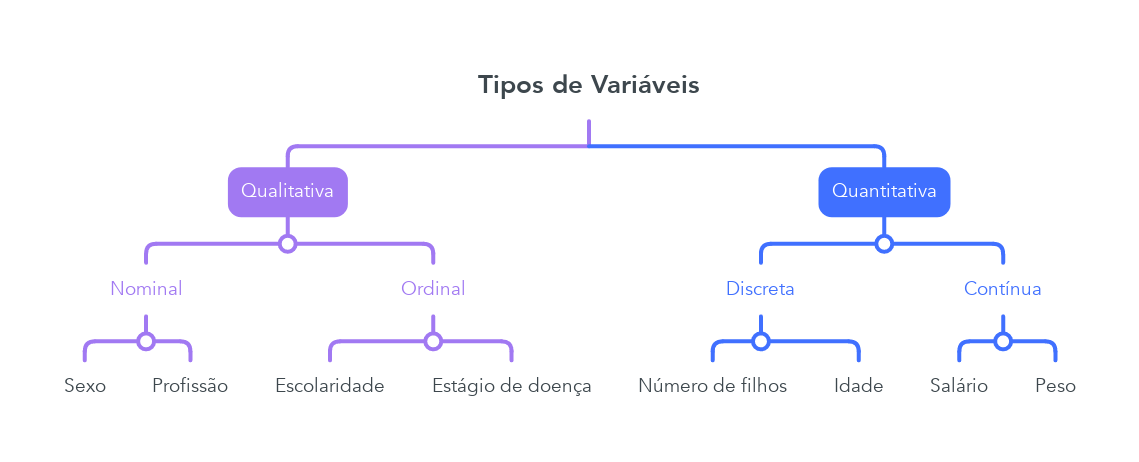
\includegraphics{figs/tipos_de_variaveis.png}
\end{itemize}

Muitas vezes queremos resumir estes dados, apresentando um ou mais valores que sejam representativos da série toda. Neste contexto entram às \textbf{medidas de posição e dispersão}.

\hypertarget{medidas-de-posiuxe7uxe3o}{%
\section{Medidas de Posição}\label{medidas-de-posiuxe7uxe3o}}

Usualmente utilizamos uma das seguintes medidas de posição (ou localização): \textbf{média, mediana ou moda}. Vamos as suas definições:

\begin{itemize}
\item
  \textbf{Moda:} valor mais frequente do conjunto de valores observados.
\item
  \textbf{Mediana:} valor que ocupa a posição central das observações quando estas estão ordenadas em ordem crescente.

  \begin{itemize}
  \tightlist
  \item
    Quando o número de observações for par, usa-se como mediana a média aritmética das duas observações centrais.
  \end{itemize}
\end{itemize}

Na tabela \ref{tab:youtubers} temos a seguinte mediana para uma coluna específica:

\begin{Shaded}
\begin{Highlighting}[]
\FunctionTok{median}\NormalTok{(df}\SpecialCharTok{$}\NormalTok{salario)}
\end{Highlighting}
\end{Shaded}

\begin{verbatim}
## [1] 4500
\end{verbatim}

Para todas as colunas:

\begin{Shaded}
\begin{Highlighting}[]
\CommentTok{\# Aplicaremos a função median para todas as colunas:}
\FunctionTok{apply}\NormalTok{(df, }\AttributeTok{MARGIN =} \DecValTok{2}\NormalTok{, }\AttributeTok{FUN =}\NormalTok{ median)}
\end{Highlighting}
\end{Shaded}

\begin{verbatim}
##            nome       est_civil    escolaridade        n_filhos         salario 
##          "Leon"        "Casado" "Pós-graduação"             "0"          "4500" 
##           idade 
##            "33"
\end{verbatim}

\begin{itemize}
\item
  \textbf{Média:} soma de todos os elementos do conjunto dividida pela quantidade de elementos do conjunto

  \[
  \overline{x} = \frac{x_1+x_2 + \dots + x_n}{n}
  \]
\end{itemize}

Na tabela \ref{tab:youtubers} temos a seguinte mediana para uma coluna específica:

\begin{Shaded}
\begin{Highlighting}[]
\FunctionTok{mean}\NormalTok{(df}\SpecialCharTok{$}\NormalTok{salario)}
\end{Highlighting}
\end{Shaded}

\begin{verbatim}
## [1] 3900
\end{verbatim}

Para todas as colunas:

\begin{Shaded}
\begin{Highlighting}[]
\FunctionTok{colMeans}\NormalTok{(df[, }\FunctionTok{c}\NormalTok{(}\StringTok{\textquotesingle{}idade\textquotesingle{}}\NormalTok{, }\StringTok{\textquotesingle{}salario\textquotesingle{}}\NormalTok{)])}
\end{Highlighting}
\end{Shaded}

\begin{verbatim}
##   idade salario 
##    33.2  3900.0
\end{verbatim}

\hypertarget{medidas-de-dispersuxe3o}{%
\section{Medidas de Dispersão}\label{medidas-de-dispersuxe3o}}

O resumo de um conjunto de dados por uma única medida representativa de posição esconde toda a informação sobre a variabilidade de um conjunto de observações. Consideremos que cinco alunos realizaram cinco provas, obtendo as seguintes notas:

\begin{Shaded}
\begin{Highlighting}[]
\NormalTok{nomes }\OtherTok{=} \FunctionTok{c}\NormalTok{(}\StringTok{\textquotesingle{}alunoA\textquotesingle{}}\NormalTok{, }\StringTok{\textquotesingle{}alunoB\textquotesingle{}}\NormalTok{, }\StringTok{\textquotesingle{}alunoC\textquotesingle{}}\NormalTok{,}
          \StringTok{\textquotesingle{}alunoD\textquotesingle{}}\NormalTok{, }\StringTok{\textquotesingle{}alunoE\textquotesingle{}}\NormalTok{)}
\NormalTok{notas }\OtherTok{=} \FunctionTok{matrix}\NormalTok{(}\FunctionTok{c}\NormalTok{(}\DecValTok{3}\NormalTok{,}\DecValTok{4}\NormalTok{,}\DecValTok{5}\NormalTok{,}\DecValTok{6}\NormalTok{,}\DecValTok{7}\NormalTok{,}
               \DecValTok{1}\NormalTok{,}\DecValTok{3}\NormalTok{,}\DecValTok{5}\NormalTok{,}\DecValTok{7}\NormalTok{,}\DecValTok{9}\NormalTok{,}
               \DecValTok{2}\NormalTok{,}\DecValTok{5}\NormalTok{,}\DecValTok{5}\NormalTok{,}\DecValTok{5}\NormalTok{,}\DecValTok{8}\NormalTok{,}
               \DecValTok{3}\NormalTok{,}\DecValTok{5}\NormalTok{,}\DecValTok{5}\NormalTok{,}\DecValTok{5}\NormalTok{,}\DecValTok{7}\NormalTok{,}
               \DecValTok{0}\NormalTok{,}\DecValTok{0}\NormalTok{,}\DecValTok{5}\NormalTok{,}\DecValTok{10}\NormalTok{,}\DecValTok{10}\NormalTok{), }\AttributeTok{nrow =} \DecValTok{5}\NormalTok{, }\AttributeTok{ncol =} \DecValTok{5}\NormalTok{, }\AttributeTok{byrow =}\NormalTok{ T)}
\NormalTok{df }\OtherTok{=} \FunctionTok{data.frame}\NormalTok{(notas, }\AttributeTok{row.names =}\NormalTok{ nomes)}
\FunctionTok{colnames}\NormalTok{(df) }\OtherTok{=} \FunctionTok{c}\NormalTok{(}\StringTok{\textquotesingle{}P1\textquotesingle{}}\NormalTok{, }\StringTok{\textquotesingle{}P2\textquotesingle{}}\NormalTok{, }\StringTok{\textquotesingle{}P3\textquotesingle{}}\NormalTok{, }\StringTok{\textquotesingle{}P4\textquotesingle{}}\NormalTok{, }\StringTok{\textquotesingle{}P5\textquotesingle{}}\NormalTok{)}
\FunctionTok{kable}\NormalTok{(df, }\AttributeTok{align =} \StringTok{\textquotesingle{}c\textquotesingle{}}\NormalTok{)}
\end{Highlighting}
\end{Shaded}

\begin{tabular}{l|c|c|c|c|c}
\hline
  & P1 & P2 & P3 & P4 & P5\\
\hline
alunoA & 3 & 4 & 5 & 6 & 7\\
\hline
alunoB & 1 & 3 & 5 & 7 & 9\\
\hline
alunoC & 2 & 5 & 5 & 5 & 8\\
\hline
alunoD & 3 & 5 & 5 & 5 & 7\\
\hline
alunoE & 0 & 0 & 5 & 10 & 10\\
\hline
\end{tabular}

Temos as seguintes médias para os alunos:

\begin{Shaded}
\begin{Highlighting}[]
\FunctionTok{rowMeans}\NormalTok{(df)}
\end{Highlighting}
\end{Shaded}

\begin{verbatim}
## alunoA alunoB alunoC alunoD alunoE 
##      5      5      5      5      5
\end{verbatim}

Cada aluno possui a mesma média de notas, porém, isto não informa nada sobre a diferença na \textbf{variabilidade das notas.} A partir disto, são criadas medidas que sumarizam a \textbf{variabilidade} de um conjunto de observações.

Em um primeiro momento podemos podemos considerar a soma da diferença dos dados em relação a média:

\[
x_1 - \overline{x} + x_2 - \overline{x} + \cdots + x_n - \overline{x}
\]

Porém, em qualquer conjunto a soma destes desvios é igual a zero. Uma alterntiva é então adicionar o valor absoluto em cada diferença:

\[
|x_1 - \overline{x}| + |x_2 - \overline{x}| + \cdots + |x_n - \overline{x}|
\]

Apesar de possuir uma boa interpretabilidade, tal métrica não possui propriedades matemáticas interessantes. Assim, trabalharemos com a diferença de quadrados de um conjunto de dados:

\[
(x_1 - \overline{x})^2 + (x_2 - \overline{x})^2 + \cdots + (x_n - \overline{x})^2
\]

Como muitas vezes queremos comparar conjuntos de dados de diferentes tamanhos, realizamos a divisão destes valores pelo total de elementos em uma amostra:

\[
\text{var}(X) = \frac{(x_1 - \overline{x})^2 + (x_2 - \overline{x})^2 + \cdots + (x_n - \overline{x})^2}{n}
\]

A partir disto, definimos \textbf{desvio padrão} como sendo a raiz da variância:

\[
\text{dp} = \sqrt{\text{var}(X)}
\]

Realizamos isto pois caso os dados estejam em uma certa unidade de medida, como \(cm\) , ao calcularmos a variância passamos a trabalhar com \(cm^2\), o que dificulta a interpretabilidade dos resultados.

\hypertarget{quantis-empuxedricos}{%
\section{Quantis Empíricos}\label{quantis-empuxedricos}}

Tanto a \textbf{média} como o \textbf{desvio padrão} podem não ser medidas adequadas para representar um conjunto de dados, uma vez que:

\begin{itemize}
\item
  São afetados por valores extremos;
\item
  Apenas os dois valores não dão informação sobre a simetria ou assimetria da distribuição dos dados
\end{itemize}

Vimos que a \textbf{mediana} é define uma divisão dos dados em duas metades. Além disto existem medidas chamadas de \textbf{quantil de ordem p} ou \textbf{p-quantil} indicado por \(q(p)\) onde \(p\) é uma proporção qualquer, \(0<p<1\) tal que \(100\%\) das observações sejam menores do que \(q(p)\).

Abaixo temos alguns dos quantis mais utilizados:

\begin{itemize}
\item
  \(q(0.25) = q_1:\) \textbf{1° Quartil} ou \textbf{25° Percentil}
\item
  \(q(0.50) = q_2:\) \textbf{2° Quartil}, \textbf{Mediana} ou \textbf{50° Percentil}
\item
  \(q(0.75) = q_3:\) \textbf{3° Quartil} ou \textbf{75° Percentil}
\item
  \(q(0.40) 1:\) \textbf{4° Decil}
\item
  \(q(0.95):\) \textbf{95° Percentil}
\end{itemize}

\hypertarget{box-plot}{%
\section{Box Plot}\label{box-plot}}

A informação contida nos quantis pode ser confusa quando estamos observando vários conjuntos de dados. A partir disto traduzimos-a em um diagrama, qual é chamado de \textbf{box plot:}

Para construção dessa gráfico definimos por \textbf{intervalo interquartil} o valor:

\[
\text{IQR}(X) = q_3 - q_1
\]

Desenhamos um retângulo que parte do primeiro quartil até o terceiro, com a mediana sendo representada por uma linha em seu interior. A partir do retângulo desenhamos uma linha até o maior ponto que não exceta o valor \(q_3+1.5 \cdot \text{IQR}(X)\), chamado de limite superior. De modo análogo fazemos o mesmo procedimento até a parte inferior do retângulo considerando o valor \(q_1 + 1.5 \cdot \text{IQR}(X)\) chamado de limite interior. As observações que estiverem acima do limite superior ou abaixo do limite superior são chamados de pontos exteriores e representadas por asteriscos. Essas observações podem ser chamaas de outliers ou valores atípicos.

O \textbf{box plot} dá uma ideia de posição, dispersão, assimetria dos dados.

\hypertarget{transformauxe7uxf5es}{%
\section{Transformações}\label{transformauxe7uxf5es}}

Vários procedimentos estatísticos são baseados na posição que os dados possuem uma distribuição em forma de sino (oriundos de uma distribuição normal), ou que a distribuição seja mais ou menos simétrica.

Se quisermos utilizar tais procedimentos podemos efetuar transformações nas observações, de modo a se obter uma distribuição mais simétrica e próxima da normal. As transformações mais frequentemente utilizadas são:

\[
x = \left\{\begin{matrix}&\sqrt{x}\\ &\ln(x) \\&\frac{1}{x}\end{matrix}\right.
\]

para cada transformação obtemos gráficos apropriados para os dados originais e transformados, de modo a escolhermos o valor mais adequado de \(p\).

\hypertarget{lab-01---conjunto-de-dados-iris}{%
\section{Lab 01 - Conjunto de dados Iris}\label{lab-01---conjunto-de-dados-iris}}

O conjunto de dados Iris é um dos mais utilizados quando introduzimos conceitos de ciência de dados. Este pode ser encontrado em \href{http://archive.ics.uci.edu/ml/index.php}{UCI Machine Learning Repository}. Tal conjunto consiste de 150 amostras de 4 tipos de espécies de flores distintas contendo os atributos:

\begin{itemize}
\item
  SepalLengthCm
\item
  SepalWidthCm
\item
  PetalLengthCm
\item
  PetalWidthCm
\end{itemize}

Podemos acessá-lo no R sem nenhum carregamento prévio da seguinte forma:

\begin{Shaded}
\begin{Highlighting}[]
\CommentTok{\# A função head() mostra os cinco primeiros itens de data.frame:}
\FunctionTok{head}\NormalTok{(iris)}
\end{Highlighting}
\end{Shaded}

\begin{verbatim}
##   Sepal.Length Sepal.Width Petal.Length Petal.Width Species
## 1          5.1         3.5          1.4         0.2  setosa
## 2          4.9         3.0          1.4         0.2  setosa
## 3          4.7         3.2          1.3         0.2  setosa
## 4          4.6         3.1          1.5         0.2  setosa
## 5          5.0         3.6          1.4         0.2  setosa
## 6          5.4         3.9          1.7         0.4  setosa
\end{verbatim}

Há certas boas práticas ao carregar um conjunto de dados, dentre elas temos:

\begin{itemize}
\item
  Visualização de sua dimensão:

\begin{Shaded}
\begin{Highlighting}[]
\CommentTok{\# O primeiro valor é a quantidade de linhas do conjunto de dados}
\CommentTok{\# e o segundo a sua quantidade de atributos}
\FunctionTok{dim}\NormalTok{(iris)}
\end{Highlighting}
\end{Shaded}

\begin{verbatim}
## [1] 150   5
\end{verbatim}
\item
  Visualização do tipo de cada atributo:

\begin{Shaded}
\begin{Highlighting}[]
\FunctionTok{str}\NormalTok{(iris) }\CommentTok{\# Structure of an Arbitrary R Object}
\end{Highlighting}
\end{Shaded}

\begin{verbatim}
## 'data.frame':    150 obs. of  5 variables:
##  $ Sepal.Length: num  5.1 4.9 4.7 4.6 5 5.4 4.6 5 4.4 4.9 ...
##  $ Sepal.Width : num  3.5 3 3.2 3.1 3.6 3.9 3.4 3.4 2.9 3.1 ...
##  $ Petal.Length: num  1.4 1.4 1.3 1.5 1.4 1.7 1.4 1.5 1.4 1.5 ...
##  $ Petal.Width : num  0.2 0.2 0.2 0.2 0.2 0.4 0.3 0.2 0.2 0.1 ...
##  $ Species     : Factor w/ 3 levels "setosa","versicolor",..: 1 1 1 1 1 1 1 1 1 1 ...
\end{verbatim}
\item
  Sumário de seus atributos:

\begin{Shaded}
\begin{Highlighting}[]
\FunctionTok{summary}\NormalTok{(iris)}
\end{Highlighting}
\end{Shaded}

\begin{verbatim}
##   Sepal.Length    Sepal.Width     Petal.Length    Petal.Width   
##  Min.   :4.300   Min.   :2.000   Min.   :1.000   Min.   :0.100  
##  1st Qu.:5.100   1st Qu.:2.800   1st Qu.:1.600   1st Qu.:0.300  
##  Median :5.800   Median :3.000   Median :4.350   Median :1.300  
##  Mean   :5.843   Mean   :3.057   Mean   :3.758   Mean   :1.199  
##  3rd Qu.:6.400   3rd Qu.:3.300   3rd Qu.:5.100   3rd Qu.:1.800  
##  Max.   :7.900   Max.   :4.400   Max.   :6.900   Max.   :2.500  
##        Species  
##  setosa    :50  
##  versicolor:50  
##  virginica :50  
##                 
##                 
## 
\end{verbatim}
\end{itemize}

Dessa maneira poderemos contatar valores errôneos no conjunto de dados, distribuições de variáveis categóricas e ter um melhor contato com o conjunto de dados.

Há ainda diversas maneiras de realizarmos visualizações desse conjunto no \texttt{R}, observemos o boxplot da variável Sepa.Length:

\begin{Shaded}
\begin{Highlighting}[]
\FunctionTok{boxplot}\NormalTok{(iris}\SpecialCharTok{$}\NormalTok{Sepal.Length)}
\end{Highlighting}
\end{Shaded}

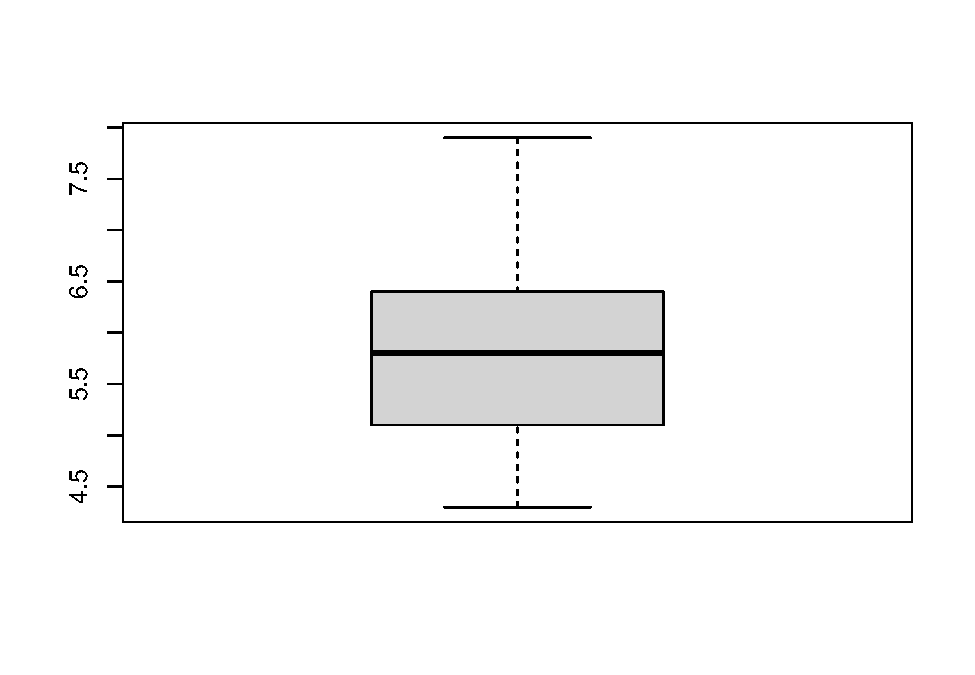
\includegraphics{_main_files/figure-latex/unnamed-chunk-19-1.pdf}

\begin{Shaded}
\begin{Highlighting}[]
\FunctionTok{ggplot}\NormalTok{(}\AttributeTok{data =}\NormalTok{ iris, }\FunctionTok{aes}\NormalTok{(}\AttributeTok{y =}\NormalTok{ Sepal.Length)) }\SpecialCharTok{+}
  \FunctionTok{geom\_boxplot}\NormalTok{() }\SpecialCharTok{+}
  \FunctionTok{labs}\NormalTok{(}\AttributeTok{title =} \StringTok{\textquotesingle{}Boxplot Iris\textquotesingle{}}\NormalTok{) }\SpecialCharTok{+}
  \FunctionTok{theme}\NormalTok{(}\AttributeTok{axis.ticks.x =} \FunctionTok{element\_blank}\NormalTok{(),}
  \AttributeTok{axis.text.x =} \FunctionTok{element\_blank}\NormalTok{())}
\end{Highlighting}
\end{Shaded}

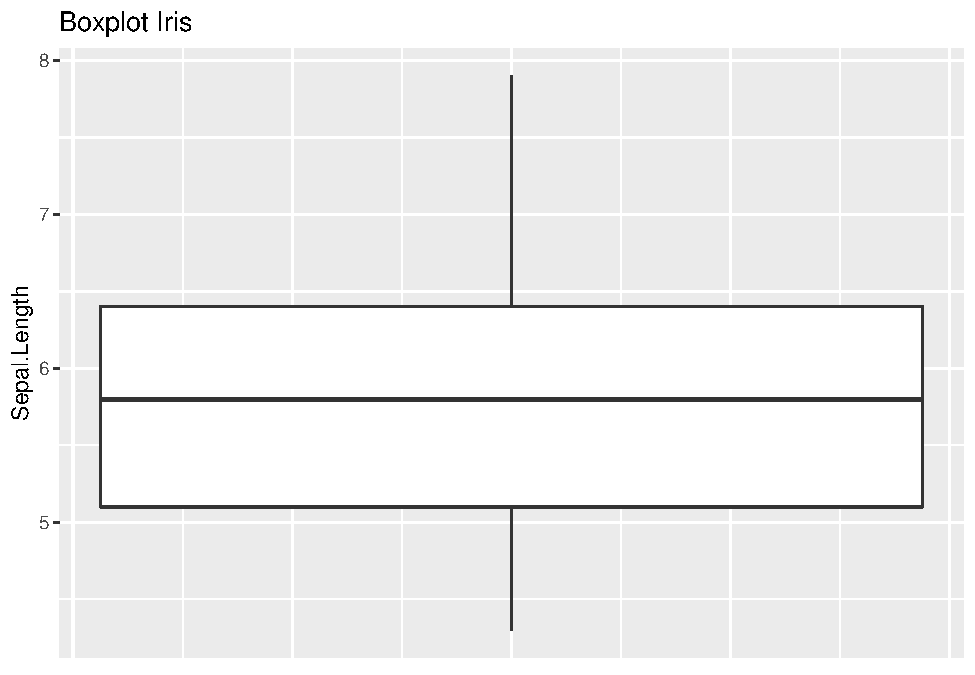
\includegraphics{_main_files/figure-latex/unnamed-chunk-20-1.pdf}

Observamos que não há presença de outliers, além disso, como a parte debaixo do retângulo separado pela linha que representa a mediana é menor, isto indica que a distribuição dos dados é ligeiramente assimétrica, o qual é confirmado pelo histograma:

\begin{Shaded}
\begin{Highlighting}[]
\FunctionTok{hist}\NormalTok{(iris}\SpecialCharTok{$}\NormalTok{Sepal.Length)}
\end{Highlighting}
\end{Shaded}

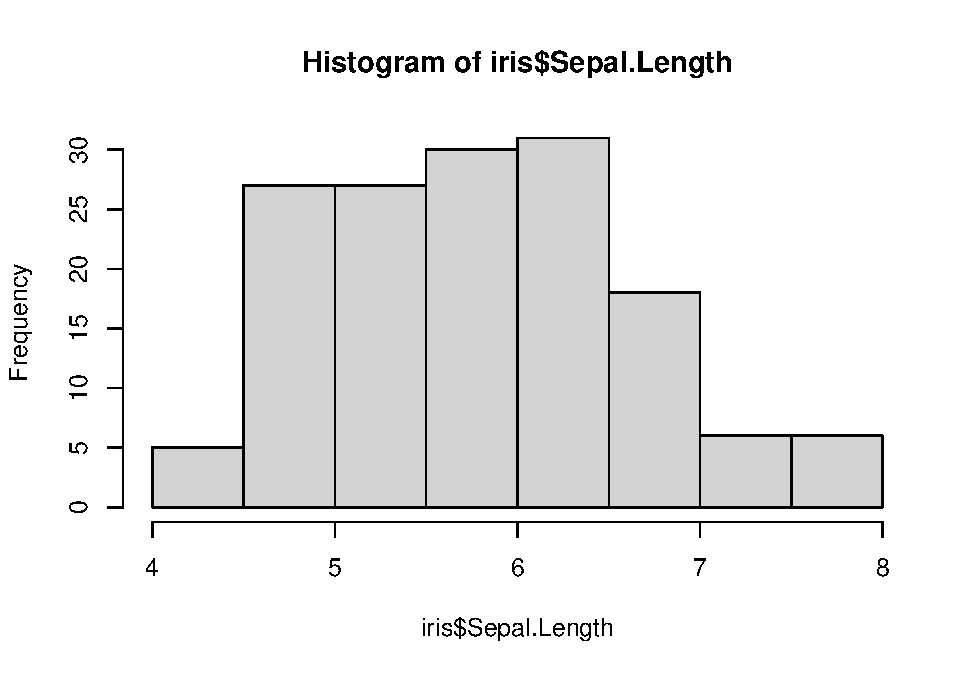
\includegraphics{_main_files/figure-latex/unnamed-chunk-21-1.pdf}

\begin{Shaded}
\begin{Highlighting}[]
\FunctionTok{ggplot}\NormalTok{(}\AttributeTok{data =}\NormalTok{ iris, }\FunctionTok{aes}\NormalTok{(}\AttributeTok{x =}\NormalTok{ Sepal.Length, }\AttributeTok{fill =}\NormalTok{ ..count..)) }\SpecialCharTok{+}
  \FunctionTok{geom\_histogram}\NormalTok{(}\AttributeTok{binwidth =} \FloatTok{0.25}\NormalTok{, }\AttributeTok{boundary =} \DecValTok{0}\NormalTok{) }\SpecialCharTok{+}
  \FunctionTok{scale\_x\_continuous}\NormalTok{(}\AttributeTok{breaks =} \FunctionTok{seq}\NormalTok{(}\DecValTok{1}\NormalTok{, }\DecValTok{10}\NormalTok{, }\AttributeTok{by =} \FloatTok{0.25}\NormalTok{)) }
\end{Highlighting}
\end{Shaded}

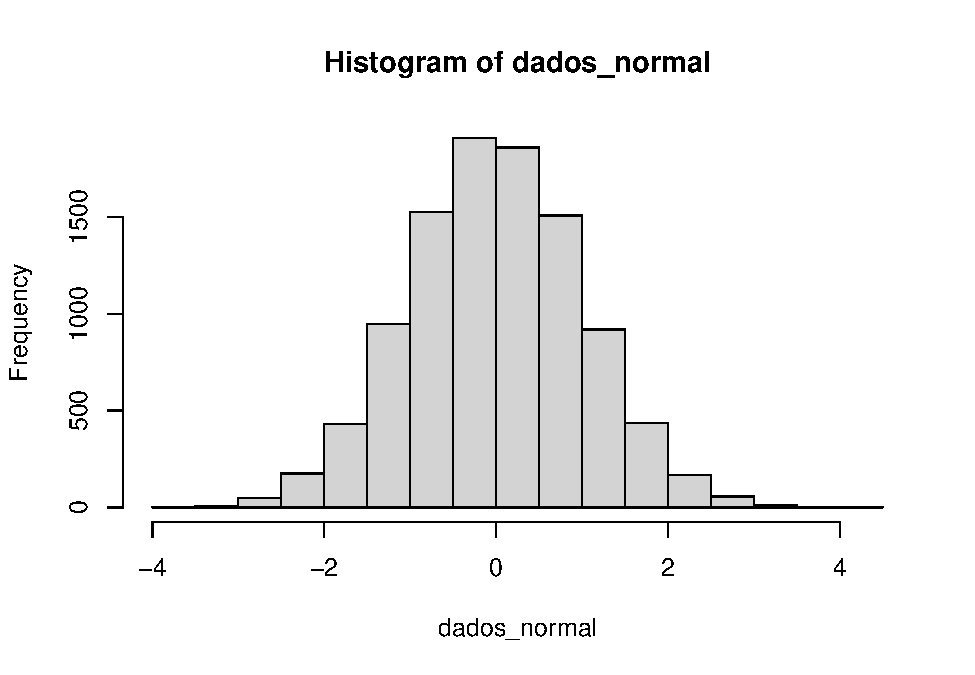
\includegraphics{_main_files/figure-latex/unnamed-chunk-22-1.pdf}

\hypertarget{tipos-de-distribuiuxe7uxf5es-discretas}{%
\chapter{Tipos de Distribuições Discretas}\label{tipos-de-distribuiuxe7uxf5es-discretas}}

Para atender a situações mais práticas, é necessário expandir os conceitos relacionados a probabilidade de forma que tenhamos modelos probabilísticos que representem todos os tipos de variáveis. Neste capítulo trabalharemos com variáveis quantativas discretas.

\begin{quote}
Exemplo (Bussab):
\end{quote}

Chamamos de \textbf{variável aleatória discreta} uma função \(X\) definida no espaço amostral \(\Omega\) que assume valores em um conjunto de números finito.

Neste contexto vimos como associar a cada valor \(x_i\) da variável aleatória \(X\) a sua probabilidade de ocorrência. Matematicamente, escrevemos

Além disso, chamamos de \textbf{função de probabilidade} da variável aleatória discreta \(X\) a função que a cada valor de \(x_i\) associa a sua probabilidade de ocorrência

\[
p(x_i) = PX=x_i) = p_i, i =1, 2, \dots
\]

\hypertarget{valor-muxe9dio-de-uma-variuxe1vel-aleatuxf3ria}{%
\section{Valor Médio de uma Variável Aleatória}\label{valor-muxe9dio-de-uma-variuxe1vel-aleatuxf3ria}}

Dada uma variável aleatórai \(X\) discreta, assumindo os valores \$x\_1,\textbackslash dots, x\_n\$, chamamos de valor médio ou esperança de \(X\) o valor

\[
E[X] = \sum_{i=1}^n x_i P(X=x_i) = \sum_{i=1}^n x_i p_i.
\]

Chamamos de variância da variável aleatória \(X\) o valor

\[
\text{var}[X] = \sum_{i=1}^n [x_i - E[X]]^2 p_i
\]

\hypertarget{tipos-de-distribuiuxe7uxf5es-contuxednuas}{%
\chapter{Tipos de Distribuições Contínuas}\label{tipos-de-distribuiuxe7uxf5es-contuxednuas}}

\hypertarget{introduuxe7uxe3o-as-bibliotecas-do-r}{%
\chapter{Introdução as bibliotecas do R}\label{introduuxe7uxe3o-as-bibliotecas-do-r}}

\hypertarget{dplyr}{%
\section{Dplyr}\label{dplyr}}

\hypertarget{tidyr}{%
\section{Tidyr}\label{tidyr}}

\hypertarget{ggplot2}{%
\section{GGPlot2}\label{ggplot2}}

\hypertarget{regressuxe3o-linear}{%
\chapter{Regressão Linear}\label{regressuxe3o-linear}}

  \bibliography{book.bib,packages.bib}

\end{document}
